\documentclass[12pt]{article}

\usepackage[english]{babel}
\usepackage[utf8x]{inputenc}
\usepackage{amsmath}
\usepackage{graphicx}
\usepackage[colorinlistoftodos]{todonotes}
\usepackage[english]{babel}
\usepackage[utf8x]{inputenc}

\DeclareGraphicsExtensions{.pdf}
\title{Sharing Framework}
\author{Chris Spalding, Wesley Stedman, Bobby Kearns, Greg Finch}
\date{\today}

\begin{document}
\maketitle

\subsection{Abstract}
\textit{The Sharing Framework is implementing a database to allow users to save and share projects that they're working on. The team's use cases deal with logging on, uploading projects, saving projects, and sharing projects. Some functional requirements include what systems Edith with support as well as what might happen if the server is over capacity.}

\section{Introduction}
Edith is a code editor aimed at beginning computer programers. It uses visual tools to help coders conceptualize what the computer and code are doing when they `write' their programs.

The Sharing Framework team is implementing a database to store the projects that are created using Edith. The database will be able to store a user's account information, as well as allow them to save and continually edit projects that are connected to their account. Along with this, the database will help with implementing the functionality that allows users to share their projects. Without the database that can save and store a user's project, no user's would be able to save a project that was too large or time consuming to finish in one sitting, making Edith a much less useful tool.
\newpage
\section{Requirements}
\textbf{Functional Requirements and Use Cases:}
\begin{description}
\item[logging on] \hfill\\
   \textit{Actor:} User\\
  \textit{Preconditions:} none that aren’t obvious (must have a computer, internet, etc.).\\
  \textit{Flow:} First the user must enter their username and password, and then click ‘login’ or an equivalent button.\\
\textit{Alternatives:} If the user doesn’t have an account then the system will prompt the user to make an account. If the user enters the wrong username/password the system will tell user and prompt them to enter username/password again.\\
\textit{Post Conditions:}
    user is logged on and can access their profile and upload/save/share docs.
\item[Saving Animations]\hfill\\
\textit{Actor:} User\\
\textit{Preconditions:} Must be logged on. Must have network connection\\
\textit{Flow:} User names animation and then selects save.\\
\textit{Alternatives:} if the animation has the same name as another animation, system prompts user “overwrite old file or rename?”\\
\textit{Post Conditions:} the animation is saved on the server under their username.\\
\item[Sharing Animations]\hfill\\
\textit{Actor:} User\\
\textit{Preconditions/Assumptions:} User must be logged on with a connection to network and they have to have a saved animation.\\
\textit{Flow:} first log on, then select share, then select animation to share, and finally the user receives link to animation\\
\textit{Alternatives:} If the user is not logged on the system will prompt him/her to log on. If the user has no animations to share the system will throw an error mesage.\\
\textit{PostConditions:} return a link to animation and perhaps display it\\
\item[Loading From The Database]\hfill\\
\textit{Actor:} User\\
\textit{Preconditions:} The user must have an account and be logged in, have a network connection of some sort, and they must have a saved animation or project to load.\\

\textit{Flow:} The user must log on and then select which animation or project to load.\\

\textit{Alternatives:} If the user is not logged in, prompt them to do so. If there is no animations to load prompt them to start a new project.\\

\textit{Postconditions:} Display the animation and all the tools needed to share or edit.\\
\end{description}

\textbf{Nonfunctional Requirements}
\begin{description}
\item[Network Connection]\hfill\\
    A strong network connection between client and server is required for the functions to properly occur.
\item[Server Overuse]\hfill\\
    If too many users are making requests, the server may not be able to respond in a timely manner or even at all.
\item[What Systems We Will Support]\hfill\\
    This program will not support mobile devices.
\end{description}

On the next page you can find the UML diagram for the use cases described above.

\begin{center}
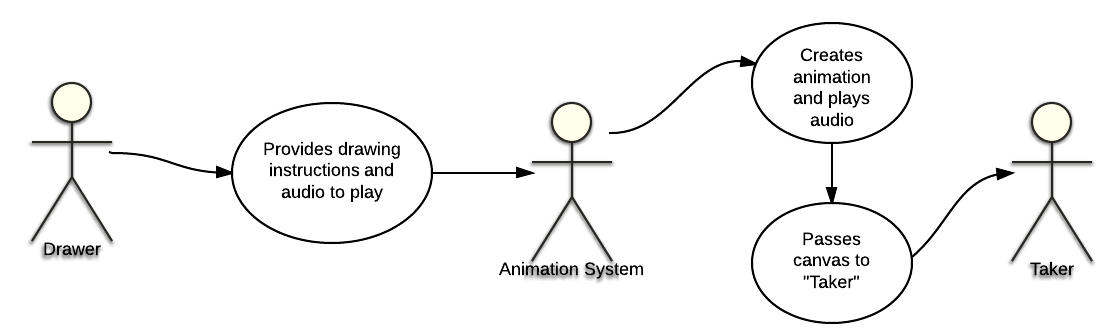
\includegraphics[scale=1]{UML}
\end{center}

\end{document}